\section{Preliminaries}
\begin{frame}
    A signed degree sequence is in \textit{standard form} if $p > d_1 \geq d_2 \geq \cdots \geq d_n$ and $d_1 \geq |d_p|$.

    We can put any sequence into standard form via the following procedure.

    \begin{enumerate}
        \item Order the elements of the sequence in descending order.
        \item If $d_1 \leq |d_n|$, multiply the sequence by $-1$ and reverse the order.
    \end{enumerate}
\end{frame}

\begin{frame}
    \begin{figure}[H]
        \centering
        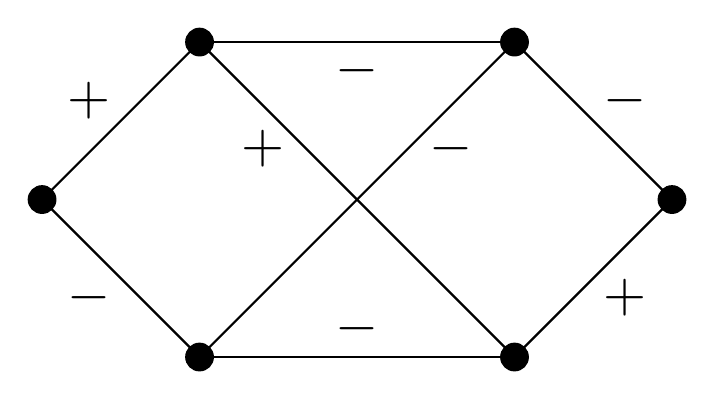
\begin{tikzpicture}[scale=1]
            %graph
            \draw[thick] (2,2)--(4,0);

            \node[right] at (3,1.25) {\(\scalebox{2}{\(-\)}\)};
    
            \draw[thick] (4,0)--(2,-2);

            \node[right] at (3,-1.25) {\(\scalebox{2}{\(+\)}\)};
    
            \draw[thick] (2,-2)--(-2,-2);

            \node[above] at (0,-2) {\(\scalebox{2}{\(-\)}\)};
    
            \draw[thick] (-2,-2)--(-4,0);

            \node[left] at (-3,-1.25) {\(\scalebox{2}{\(-\)}\)};
    
            \draw[thick] (-4,0)--(-2,2);

            \node[left] at (-3,1.25) {\(\scalebox{2}{\(+\)}\)};
    
            \draw[thick] (-2,2)--(2,2);

            \node[below] at (0,2) {\(\scalebox{2}{\(-\)}\)};
    
            \draw[thick] (-2,2)--(2,-2);

            \node[below] at (1.2,1) {\(\scalebox{2}{\(-\)}\)};
    
            \draw[thick] (2,2)--(-2,-2);

            \node[below] at (-1.2,1) {\(\scalebox{2}{\(+\)}\)};
    
            \draw[fill] (-2,2) circle (5pt);
    
            \draw[fill] (2,2) circle (5pt);
    
            \draw[fill] (4,0) circle (5pt);
    
            \draw[fill] (2,-2) circle (5pt);
    
            \draw[fill] (-2,-2) circle (5pt);
    
            \draw[fill] (-4,0) circle (5pt);
        \end{tikzpicture}
    \end{figure}
    \begin{equation*}
        \sigma : 1, -3, 0, 1, -3, 0 \to 1,1,0,0,-3,-3
    \end{equation*}
\end{frame}

\begin{frame}
    \begin{figure}[H]
        \centering
        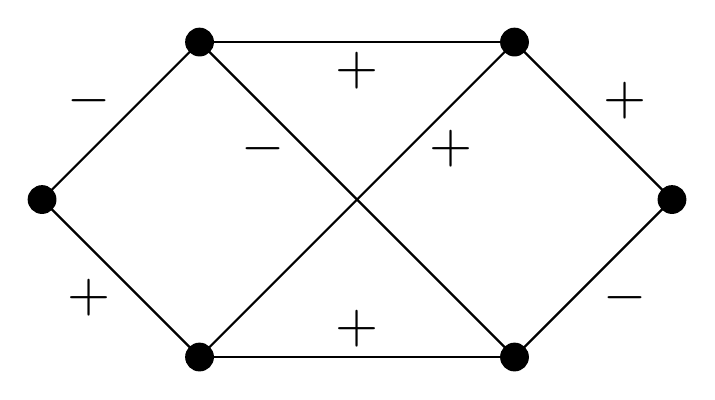
\begin{tikzpicture}[scale=1]
            %graph
            \draw[thick] (2,2)--(4,0);

            \node[right] at (3,1.25) {\(\scalebox{2}{\(+\)}\)};
    
            \draw[thick] (4,0)--(2,-2);

            \node[right] at (3,-1.25) {\(\scalebox{2}{\(-\)}\)};
    
            \draw[thick] (2,-2)--(-2,-2);

            \node[above] at (0,-2) {\(\scalebox{2}{\(+\)}\)};
    
            \draw[thick] (-2,-2)--(-4,0);

            \node[left] at (-3,-1.25) {\(\scalebox{2}{\(+\)}\)};
    
            \draw[thick] (-4,0)--(-2,2);

            \node[left] at (-3,1.25) {\(\scalebox{2}{\(-\)}\)};
    
            \draw[thick] (-2,2)--(2,2);

            \node[below] at (0,2) {\(\scalebox{2}{\(+\)}\)};
    
            \draw[thick] (-2,2)--(2,-2);

            \node[below] at (1.2,1) {\(\scalebox{2}{\(+\)}\)};
    
            \draw[thick] (2,2)--(-2,-2);

            \node[below] at (-1.2,1) {\(\scalebox{2}{\(-\)}\)};
    
            \draw[fill] (-2,2) circle (5pt);
    
            \draw[fill] (2,2) circle (5pt);
    
            \draw[fill] (4,0) circle (5pt);
    
            \draw[fill] (2,-2) circle (5pt);
    
            \draw[fill] (-2,-2) circle (5pt);
    
            \draw[fill] (-4,0) circle (5pt);
        \end{tikzpicture}
    \end{figure}
    \begin{align*}
        \sigma : 3, 3, 0, 0, -1, -1 \to -1, 3, 0, -1, 3, 0
    \end{align*}
\end{frame}

\begin{frame}
    This is formalized in the following result.

    \begin{lemma}
        If $\sigma : d_1,d_2,\dots d_n$ is the signed degree sequence of a signed graph $G$, then $\sigma' : -d_1,-d_2,\dots,-d_n$ is the signed degree sequence of the signed graph $G'$ which is $G$ with the sign of every edge reversed.
    \end{lemma}
\end{frame}
